% !TeX spellcheck = de_CH_frami

\section{Graph Spektralanalyse\label{sec:sgwt:spectralanalysis}}
\rhead{Graph Spektralanalyse}

Nachdem wir nun die Grundlagen von Graphen und den Laplace Operator sowie die 
Laplace Matrix angeschaut haben, wollen wir uns nun der Spektralanalyse eines 
Graphen und dann der Spektral Graph Wavelet Transformation widmen.

\subsection{Graph Fourier Transformation\label{subsec:sgwt:gft}}

Betrachten wir erst die Fouriertransformation. Bei dieser gehen wir von einem 
unendlichen langem periodischen Signal aus. Obwohl das meist nicht als solches 
vorliegt, da unsere Messungen in der Zeit beschr\"ankt sind. Dabei wird dann 
ein kleiner Trick angewendet, indem man einfach das gemessene Signal nimmt und 
es vorne und hinten ankn\"upft. Bei Wavelets kann man das nat\"urlich nicht so 
machen, da wir ja eine gewisse Lokalisierung erreichen wollen, das mit so einem 
zusammengesetzten Signal nicht mehr sinnvoll w\"are. Analog dem Ankn\"upfen des 
Signals, k\"onnen wir bei einem Liniengraphen einfach den Start- und Endknoten 
verbinden und erhalten somit ein unendlich langes periodisches Signal, 
siehe~\cref{fig:sgwt:spectrum:ring}.

\begin{figure}
    \centering
    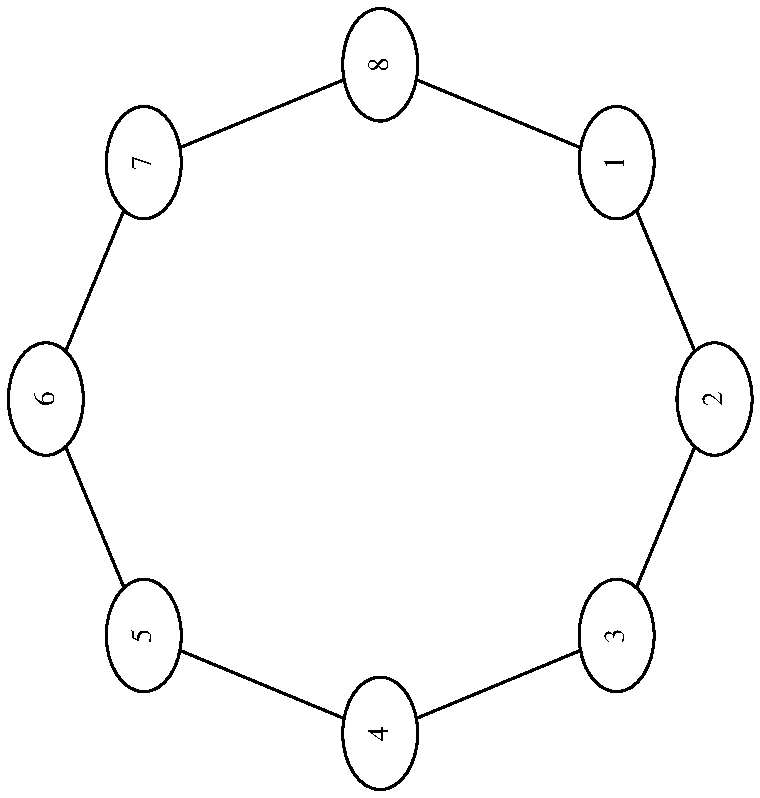
\includegraphics[
    angle=-90,
    origin=c,
    scale=0.6
    ]{papers/sgwt/images/ring-graph.pdf}
    \vspace{-10pt}
    \caption{Approximation einer periodisch erweiterten Funktion.
        \label{fig:sgwt:spectrum:ring}}
\end{figure}

\subsection{Graph Wavelet Transformation\label{subsec:sgwt:gwt}}

\begin{figure}
    \centering
    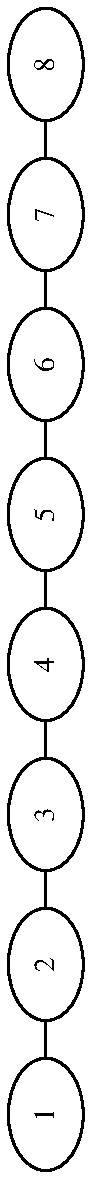
\includegraphics[
    angle=-90,
    origin=c,
    scale=0.6
    ]{papers/sgwt/images/line-graph.pdf}
    \vspace{-160pt}
    \caption{Graph Approximation einer eindimensionalen Funktion. 
        \label{fig:sgwt:spectrum:line}}
\end{figure}

\begin{figure}
    \centering
    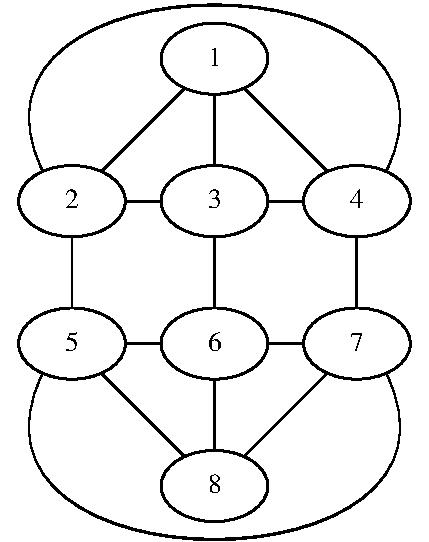
\includegraphics[
    scale=0.6
    ]{papers/sgwt/images/sphere-graph.pdf}
    \caption{Graph Approximation einer Kugel.
        \label{fig:sgwt:spectrum:sphere}}
\end{figure}

\begin{equation}
\psi_j = \chi \diag{g(\lambda)} \chi'
\end{equation}
